Single Shot MultiBox Detector (SSD), \cite{DBLP:journals/corr/LiuAESR15}, je detektor koji detektira više objekata u jednom prolazu i brži je od prve inačice detektora YOLO, a precizan kao Faster R-CNN. 
Sastoji se od duboke konvolucijske mreže koja na izlazu daje skup detekcija konstantne veličine. Raniji slojevi mreže su temeljeni na arhitekturi mreže za klasifikaciju objekata VGG16, na koje su dodani pomoćni slojevi koji generiraju detekcije. Na smanjenu osnovnu mrežu se dodaju konvolucijski slojevi od kojih je svaki manji od prethodnog što omogućuje detekciju na različitim skalama. Neki modeli procesiraju slike različitih veličina, ali se korištenjem konvolucijskih slojeva različitih veličina postiže isti učinak.
Za mapu značajki dimenzija $m \times n$ na svakoj od $m \times n$ lokacija se računa izlaz. Svakoj lokaciji se pridjeljuju unaprijed odabrani prozori različitih veličina i omjera stranica, a izlazi mreže predstavljaju pomake u odnosu na te prozore. Izlaz za svaku lokaciju uključuje predikcije pomaka svih $k$ unaprijed određenih prozora i za svaki prozor vjerojatnosti pripadnosti svakom od $c$ razreda. Na svaku lokaciju mape značajki se stoga primjenjuje $(c + 4)k$ filtera što je ukupno $(c + 4)kmn$ filtera za cijelu mapu značajki. Skale unaprijed određenih prozora za svaku od $m$ mapa značajki se računaju po formuli
\[
	s_k = s_{min} + \frac{s_{max} -s_{min}}{m - 1}(k - 1), \quad k \ \epsilon \ [1, m]
\]gdje je $s_{min}$ najmanja skala, a $s_{max}$ najveća skala. U originalnom radu se koristi 0.2 za najmanju skalu, a 0.9 za najveću. Ako se omjer stranica prozora označi s $a_r$, širina prozora se računa po formuli $w_k^a = s_k \sqrt{a_r}$, a visina po formuli $w_k^a = s_k / \sqrt{a_r}$. Arhitektura modela je prikazana na slici \ref{ssd_arhitektura}.

 \begin{figure}
	\centering
	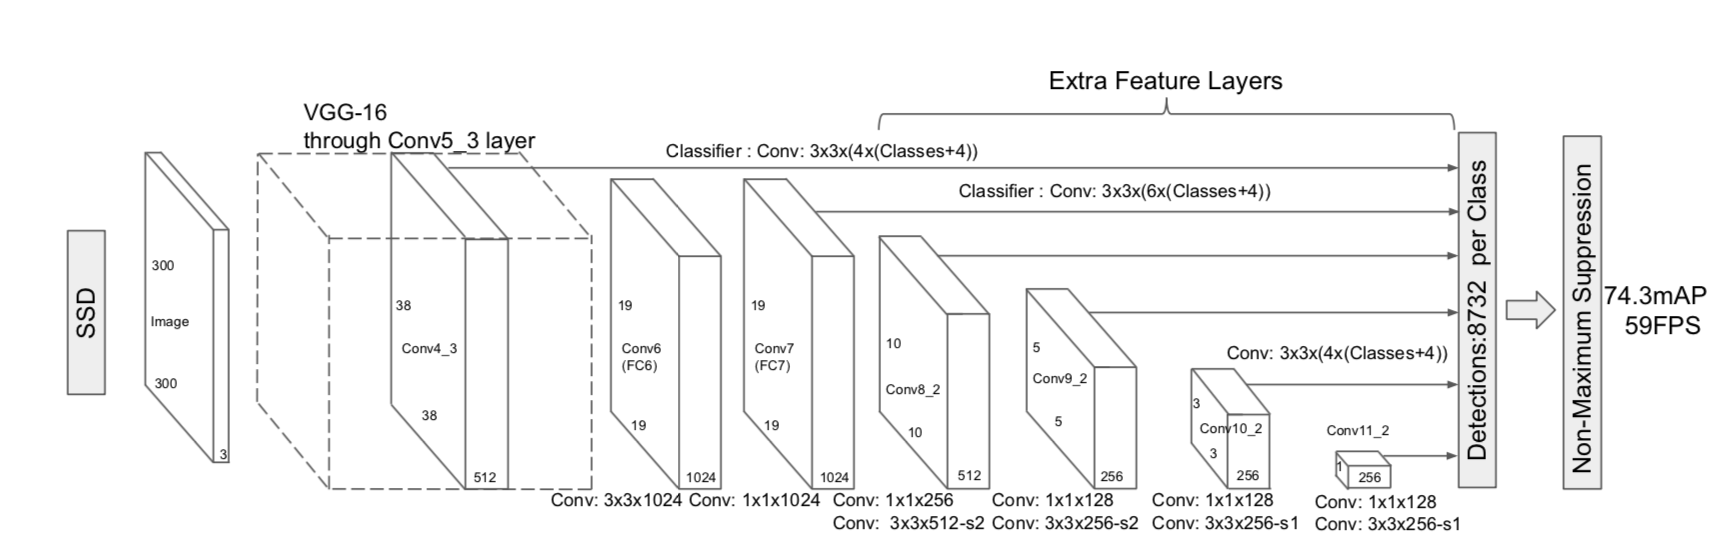
\includegraphics[scale=0.5]{img/ssd_arhitektura.png}
	\caption{Arhitektura SSD modela (\cite{DBLP:journals/corr/LiuAESR15}).}
	\label{ssd_arhitektura}
\end{figure}

Prilikom treninga je potrebno svakom unaprijed određenom prozoru pridružiti stvarni prozor objekta. Prvo se svakom stvarnom prozoru pridružuje unaprijed određeni prozor s najvećim omjerom presjeka i unije. Zatim se svakom unaprijed određenom prozoru pridružuje bilo koji stvarni prozor s kojim ima omjer presjeka i unije veći od 0.5. Time se modelu omogućuje da više unaprijed određenih prozora ima velike predviđene vjerojatnosti umjesto da se bira jedan s najvećim preklapanjem.
Nakon pridruživanja prozora, većina unaprijed određenih prozora neće biti pridruženi nijednom stvarnom prozoru pa oni čine negativne primjere. Da bi se riješio problem omjera broja negativnih i pozitivnih primjera, ne koriste se svi negativni primjeri. Negativni primjeri se sortiraju po pogrešci pouzdanosti i izaberu se primjeri s najvećom pogreškom tako da omjer broja negativnih i pozitivnih primjera ne bude veći od 3:1. 
Funkcija pogreške koja se koristi za trening modela je težinska suma lokalizacijske pogreške i pogreške pouzdanosti:
\[
	L(x, c, l, g) = \frac{1}{N}(L_{conf}(x, c) + \alpha L_{loc}(x, l, g))
\]
gdje $N$ označava broj pridruženih unaprijed određenih prozora. Ako je $N = 0$, funkcija pogreške je 0. Za lokalizacijsku pogrešku, SSD koristi zaglađeni $L_1$ kao i Faster R-CNN. Pogreška pouzdanosti je
\[
	L_{conf}(x, c) = - \sum\limits_{i \epsilon Pos}^N x^p_{ij}\log(\hat{c}^p_i) - \sum\limits_{i \epsilon Neg} \log(\hat{c}^0_i)
\]
gdje je 
\[
	\hat{c}^p_i = \frac{exp(c_i^p)}{\sum\limits_p exp(c_i^p)}
\]
Da bi model bio robusniji na različite veličine i oblike objekata, tijekom treninga se na svaku sliku nasumično primjenjuje jedna od sljedećih transformacija:
\begin{itemize}
	\item Koristi se cijela slika
	\item Nasumično se uzima uzorak slike tako da je omjer presjeka i unije uzorka s objektima na slici 0.1, 0.3, 0.5, 0.7 ili 0.9
	\item Uzima se nasumični uzorak slike
\end{itemize}
Veličina svakog uzorka je iz intervala $[0.1, 1]$ od originalne slike, a omjer stranica je između $\frac{1}{2}$ i $2$. Stvarni prozor objekta se zadržava ako njegovo središte upada u odabrani uzorak slike. 
Navedene transformacije slika povećavaju srednju preciznost modela za $8.8\%$ na skupu podataka VOC2007.